

%----------------------------------------------------------------------------------------
%	PACKAGES AND OTHER DOCUMENT CONFIGURATIONS
%----------------------------------------------------------------------------------------

\documentclass[twoside,twocolumn]{article}

\usepackage{blindtext} % Package to generate dummy text throughout this template 

\usepackage[sc]{mathpazo} % Use the Palatino font
\usepackage[T1]{fontenc} % Use 8-bit encoding that has 256 glyphs
\linespread{1.05} % Line spacing - Palatino needs more space between lines
\usepackage{microtype} % Slightly tweak font spacing for aesthetics

\usepackage[english]{babel} % Language hyphenation and typographical rules

\usepackage[hmarginratio=1:1,top=32mm,columnsep=20pt]{geometry} % Document margins
\usepackage[hang, small,labelfont=bf,up,textfont=it,up]{caption} % Custom captions under/above floats in tables or figures
\usepackage{booktabs} % Horizontal rules in tables

\usepackage{lettrine} % The lettrine is the first enlarged letter at the beginning of the text

\usepackage{enumitem} % Customized lists
\setlist[itemize]{noitemsep} % Make itemize lists more compact

\usepackage{abstract} % Allows abstract customization
\renewcommand{\abstractnamefont}{\normalfont\bfseries} % Set the "Abstract" text to bold
\renewcommand{\abstracttextfont}{\normalfont\small\itshape} % Set the abstract itself to small italic text

\usepackage{titlesec} % Allows customization of titles
\renewcommand\thesection{\Roman{section}} % Roman numerals for the sections
\renewcommand\thesubsection{\roman{subsection}} % roman numerals for subsections
\titleformat{\section}[block]{\large\scshape\centering}{\thesection.}{1em}{} % Change the look of the section titles
\titleformat{\subsection}[block]{\large}{\thesubsection.}{1em}{} % Change the look of the section titles

\usepackage{fancyhdr} % Headers and footers
\pagestyle{fancy} % All pages have headers and footers
\fancyhead{} % Blank out the default header
\fancyfoot{} % Blank out the default footer
\fancyhead[C]{Interim Report $\bullet$ \today $\bullet$ 16019243} % Custom header text
\fancyfoot[RO,LE]{\thepage} % Custom footer text

\usepackage{titling} % Customizing the title section

\usepackage{hyperref} % For hyperlinks in the PDF

\usepackage{pdfpages}

\usepackage[round]{natbib}


%----------------------------------------------------------------------------------------
%	TITLE SECTION
%----------------------------------------------------------------------------------------

\setlength{\droptitle}{-4\baselineskip} % Move the title up

\pretitle{\begin{center}\Huge\bfseries} % Article title formatting
\posttitle{\end{center}} % Article title closing formatting
\title{Parting the Clouds: working towards an affordable natural-lighting solution} % Article title
\author{%
\textsc{N. Appleton} \\[1ex] % Your name
\normalsize 16019243 \\ % Your institution
\normalsize \href{mailto:nicholas2.appleton@live.uwe.ac.uk}{nicholas2.appleton@live.uwe.ac.uk} % Your email address
}
\date{\today} % Leave empty to omit a date
\renewcommand{\maketitlehookd}{%
}

%----------------------------------------------------------------------------------------

\begin{document}

% Print the title
\maketitle

%----------------------------------------------------------------------------------------
%	ARTICLE CONTENTS
%----------------------------------------------------------------------------------------

\section{Introduction and Aims}
\label{sec:intro}

\lettrine[nindent=0em,lines=3]{F} or the past 100 years, the primary use of artificial light has been to allow people to operate beyond the scope of daylight hours. The foremost consideration, therefore, has been directed at the visual \citep{webbConsiderationsLightingBuilt2006}. However, since the turn of the 21st century, we have known that there are many non-visual effects of light, including the fact that it plays a central role in the sleep-wake cycle (or circadian rhythm) \citep{provencioNovelHumanOpsin2000, bersonPhototransductionRetinalGanglion2002}. 
There is an extensive body of research showing that bright light can delay sleep onset and have negative ramifications on sleep quality. 
Not only does light affect our sleep, but it also affects our waking experience: mood is affected largely by light exposure, as are focus, attentiveness and even cognitive performance. All these factors are influenced by the environmental light conditions to which most people don not give a second thought.
We can find the optimal light exposure for any time of day simply by looking outside: our bodies are naturally and precisely	 tuned to the cycles of the sun, and only in the past few hundred years have we forsaken these rhythms with large-scale artificial lighting.

The aims of this project are twofold: 'To produce a device that can replicate the visual output of the sun as closely as possible' and 'To validate the design by measuring the spectral output and validating the efficacy'. Further aims would be to develop the device as a product: improving the user interface and expanding its functionality. The production of the device will be split between me and Vojtěch Halenka. The completion of these goals will be made against a Product Requirements document (see appendix \ref{appendix:requirements}).

The objectives of the project, which will help achieve the aims, are to work with Vojtěch to produce a schematic that can be tested and turned into a PCB that we can get printed. With these first PCBs we can fully test our design, make any relevant changes and produce a second design from that. Once we know we have a working unit, I will be able to test the spectral output and assess the effect of the device on sleep (the research phase will be conducted independent of Vojtěch). If This is completed in a timely manner, I would also like to implement an improved UI and extra features to make the device more complete and user-friendly.


%------------------------------------------------

\section{Justification}
\label{sec:just}

The device we are producing will have the fundamental purpose of improving the health of its users. There is a wealth of knowledge demonstrating how important exposure to natural lighting patterns is on our well-being, but none of the devices currently on the market are appropriate for the problem we are trying to solve. Through a competitor review \citep{appletonCompetitorAnalysis2020}, I found that the majority of circadian lighting is for industrial (office and warehouse) use, rendering it almost pointless if the workers go home to a house equipped with standard LED lighting technologies. The few consumer grade circadian lights on the market are extortionately expensive: upwards of \$200 for a single bulb. Moreover, these can only be used in places with existing bulb fittings and therefore are not feasible for many environments. There are other devices on the market that claim to respect circadian rhythms, but many of these devices are designed either for use at specific times of day, or for `mood lighting' with circadian regulation as an option only if you ``hack'' them  - `entertainment, not entrainment' as I like to say - therefore they are not equipped with appropriate lighting for the evening hours. By creating a standalone, 12-Volt, expandable and affordable solution, we will be bringing this essential technology to many more people to whom it is not currently available.

If we look at the United Nations' Sustainable Development Goals \citep{un-desaSustainableDevelopmentGoals2016}, we can see that `Ensuring healthy lives and promoting well-being for all at all ages' is one of the goals, as is `Making cities and human settlements inclusive, safe, resilient and sustainable'. My project will try to encompass both of these goals by creating a more health-promoting, human-centric built environment that cares for the health of those exposed to its outputs. It will also be helping to reduce energy consumption by replacing outdated technologies such as incandescent and fluorescent bulbs that are both inefficient and polluting to produce and dispose of.

By making the device modular - consisting of many mix-and-match components - the user will be able to customise their device to fit their space, requiring fewer unique module designs to be produced, while still providing a scalable solution to the problem.


%------------------------------------------------

\section{Scope}
\label{sec:scope}

This project aims to deliver a works-like prototype that can be used to assess the validity of the design for use as an all-day lighting system. 
The design considerations for a final product, as well as user safety, will be observed throughout the design process.
Ideally, the final outcome will be a looks-like, works-like prototype in the form of a demonstrable unit. There are 3 main milestones for the development: completion of a functional unit, testing and validation of said unit, and furthering the design and usability once the functionality has been validated.

Doing a human trial of the effects on sleep is Out-Of-Scope of this project, both due to the ethical and resource requirements of a sleep study and due to the current pandemic. However, the effects on sleep will be assessed via	 observation of the output spectra of the device.

The current global situation of Covid-19 will have significant impacts on the completion of this project. Delivery times for components could be affected and access to equipment will be severely limited. Throughout the project, government guidance will always be followed and contingency plans put in place for each part of the project. While we are awaiting the delivery of components and PCBs, I will develop a simulator that can be used to calculate the output of the device, ensuring that I can complete the research, even if no demonstrable unit can be fabricated. The Gantt chart will also reflect this situation by allowing more time for delivery and development.

The device will be an autonomous system that requires user-input only to set parameters of the time-scale events.	It will be developed from `cradle to grave' with an emphasis on giving me a broader understanding of the tools and techniques used to design and develop systems like this to a given requirement. I hope this project will offer me a more practical experience of the design cycle and processes involved with creation of automated systems.

%------------------------------------------------

\section{Proposed Research Questions}
\label{sec:questions}

The main question that will  be researched through this project will be ``Can we can develop a device that is suitable to use throughout the day and night without negatively impacting the human cycles that we are aware of, namely the circadian rhythm?'' An additional question that will be considered throughout the project will be ``Would this device be a viable product that appeals to consumers?'' Further questions would include how people respond to using the product and whether to implement more natural variations such as `clouds' and flickering `firelight' to observe the effect this might have on users. However, it is unlikely that the scope of this project will allow for these questions to be answered - perhaps in future research.

%------------------------------------------------

\section{Initial Research}
\label{sec:research}

Electric lighting plays a large role in modern life: extending our day beyond the natural boundaries of sunset and sunrise. Our primary concern for lighting has become to provide us with accurate visual performance beyond the scope of the day - however, in recent years it has become more and more obvious that this is not optimal for human health, or even performance for that matter. 

All animals have a built in circadian rhythm that regulates their day/night cycle. This rhythm is fundamental to allow the body to effectively rest - in humans - overnight \citep{senthilnathanCircadianRhythmIts2019}. The circadian clock controls melatonin production in the brain, an important factor in the generation and quality of sleep \citep{arendtImportanceRelevanceMelatonin2003}. There are many peripheral clocks that help to set the central clock every day and keep it running on-time \citep{mohawkCentralPeripheralCircadian2012, richardsAdvancesUnderstandingPeripheral2012}. One of the most important of these cues comes from light exposure \citep{czeislerBrightLightResets1986, laaksoOnehourExposureModerate1993}, especially blue, short-wavelength light \citep{thapanActionSpectrumMelatonin2001, figueiroTrainBlueLight2013}. However, this is one of the most overlooked areas in modern built environments \citep{webbConsiderationsLightingBuilt2006}.

There are some solutions to counter this pervasive problem, for example wearing amber tinted glasses to block out the shortest wavelengths of light was shown by \cite{kimberlyAmberLensesBlock2009} to improve sleep quality. Not everyone wants to have to wear amber glasses after dark every night, especially in their own home!
Furthermore, it greatly affect one's ability to see colours accurately when wearing such glasses. Other methods include `Smart Lighting' which can be set to fade into different colours at different times, but while this may improve mood \citep{mccloughanImpactLightingMood1999}, it will not have a hugely positive effect on sleep as RGB LEDs are used to achieve the desired colour. This means the colour will almost certainly have a harmful blue component, while according to  \cite{gilewskiEcologicalHarmfulnessRGB2018}, RGB LEDs are a wholly harmful form of lighting (although this study is lax in its sources and its referencing, so perhaps should be taken with a pinch of salt). 

Older technologies, such as incandescent bulbs, produce a spectrum much closer to that of firelight \citep{f.luxsoftwarellcLuxometer}. However, they are so inefficient that they are banned from being sold in the \cite{euDirective201227}. The replacements for these technologies - Fluorescent bulbs and LEDs - have been shown to produce harmful light \citep{uedaEyeDamageControl2009, kuseDamagePhotoreceptorderivedCells2014, niwanoBlueLightInjures2014, marekBlueLightPhototoxicity2018, nakamuraExposureExcessiveBlue2018}, and many traditional bulbs of this type contain hazardous materials such as lead \citep{limPotentialEnvironmentalImpacts2013}. However, there is huge potential for LEDs to save much power in the built environment \citep{montoyaIndoorLightingTechniques2017}, but this shouldn't come at the expense of human (circadian) health. 

Another surprising impact the circadian rhythm has on our lives is in the realm of cancer; a powerful link has been demonstrated between circadian suppression and breast cancer in rats \citep{mhatreEffectVaryingPhotoperiods1984, otaloraEffectsExogenousMelatonin2008, vandenheiligenbergTumorPromotingEffect1999} and in humans - mostly observed in shift workers and flight attendants \citep{hansenIncreasedBreastCancer2001, davisNightShiftWork2001, schernhammerRotatingNightShifts2001, schernhammerNightWorkRisk2006, lieBreastCancerNight2006, tokumaruIncidenceCancerFemale2006, olearyShiftWorkLight2006, kolstadNightshiftWorkRisk2008, stevensLightatnightCircadianDisruption2009, stevensBreastCancerCircadian2014}.

It's not all bad for blue light, though. It is widely accepted that bright light is an effective treatment for Seasonal Affective Disorder (SAD) \citep{eastmanBrightLightTreatment1998, magnussonTreatmentSeasonalAffective1991} and \cite{leeSpectralPropertiesPhototherapy1997} found in their meta-analysis that shorter (blue) wavelengths appear to have a greater effect.

Furthermore, many studies have shown a positive correlation between blue light and attentiveness, cognitive performance and visual tasks throughout the day \citep{sun-youngExperimentLightingEnvironment2005, millsEffectHighCorrelated2007, lehrlBlueLightImproves2007, hawesEffectsFourWorkplace2012}. This also has been shown to be linked directly back to the circadian rhythm \citep{hawesEffectsFourWorkplace2012}.

From the evidence presented here, I hope it is clear why a product that can produce a spectrum close to that of the sun would be beneficial to people's health and well-being throughout the day, and therefore why we have decided to develop and test one.

%------------------------------------------------

\section{Methodology}
\label{sec:method}

The word methodology is defined by \cite{CollinsEnglishDictionary2014} as \emph{``a system of methods and principles for doing something, for example for teaching or for carrying out research''}. An example of this would be the the Scientific Method which is a method in which knowledge is acquired through experimentation and analysis to confirm or deny a hypothesis. 

In section \ref{sec:questions}, I discussed the proposed research questions in which I laid out my primary research question, which can be made into the hypothesis $H_1$: ``We can produce a device that can effectively be used throughout the day while avoiding a circadian phase-shift of more than 30 minutes''. This hypothesis can be tested with various tools and techniques provided by the literature and can be easily falsified, too.
This hypothesis will be investigated using quantitative methods: collecting empirical data that will be analysed to determine if the null or alternative hypothesis can be accepted.
However there are other peripheral hypotheses relating to the development of the device as a viable product. Some qualitative research would ideally take place to assess how people react to various aspects of the device which will lead to a discussion about how further development could take place, but this may be out of scope of this project due to the pandemic situation.

A more top-down view of the falsifiable points that will be used to determine whether we have succeeded in the project are laid out in the Requirements document (See appendix \ref{appendix:requirements}).

While the term `method' can easily be confused with a methodology, it refers to how the data will be collected, or how the subject will be observed. For the hypothesis $H_{1}$, experiments will be the method used to obtain the data; I will use a hyper-spectral camera to capture the spectra of the device alongside the spectra of other, similar devices. The outputs of these devices can then be compared and calibrated to more absolute values by comparing to a known source. These data will then be used to assess the efficacy of the device as a night-time light. Another method of secondary data can be used to compare the results with a broader catalogue of results gathered by others. 

For any qualitative research that were to take place, I would ideally use a participant observation and survey methods to discover people's opinions on the given research topic, but it is more feasible to just use a survey in these times.

%------------------------------------------------

\section{Project Management and Planning}
\label{sec:planning}

The project management software \cite{ClickUpProjectManagement2020} software will be used as the primary project management tool: it will contain the open, in progress and closed tasks; the Gantt chart and due dates of each deliverable, milestone and task; and documents such as my logbook and meeting minutes will be stored there.

Weekly meetings are taking place between my supervisor and me, and minutes are being kept for these meetings in my logbook. I am also having weekly meetings with V. Halenka to discuss the progress of the development phase, delegate tasks, make design decisions and consolidate new knowledge in the subject. 

The time-scale of the project has been heavily influenced by the supply chain and potential delays that may occur. As can be seen in the Gantt chart (See appendix ), we have allocated up until February for the final prototype to be ready. Work towards the research goals will happen alongside the development of the prototype - especially during the periods allocated for delivery.

The project will require more resources than some, as it involves the design and production of hardware; we will be sure to keep our minds on the sustainability of the solution by ensuring that all electronic components used are RoHS compliant. The design of the device is also modular which not only will make it more accessible, but will reduce the obsolescence of the product, as individual modules can be replaced when needed, rather than having to replace the whole unit. Another environmental implication will be the shipping of the PCBs from the factory in China to us in the UK. This is difficult to avoid as any UK-based PCB companies are well out of our budget. However, as this is a very limited production run, this could be re-assessed in the event of larger-scale production. Other resources include a hyper-spectral camera (already sourced) which does not have any upfront environmental hazard as it is already at the university. The only other identified resource that I require is software such as Matlab and LABview that are already provided by the university (See Appendix \ref{appendix:resources}).

As there are not going to be any observations made on humans, the ethical considerations will be very limited. An Ethics check-list has been completed with my supervisor to ensure that the project is ethically valid. If qualitative data is required at the later stages of the project then I will re-consider the ethical implications, as this will require thought on data-handling and management and respect of the participant's privacy and right to withdraw. If this does happen, then I will collect no personal data from the participants and all responses will be anonymised with an identification number that can be used to withdraw from the research.

This project definitely has some limitations to it: the budget is very limited for a project such as this and £75 is not enough to design and build a working prototype. Fortunately, as there are 2 of us working on the hardware, we will be able to double this budget, which should be enough to make at least a couple of demonstrable units. This project is also very limited in time: we have only 6 months to create, test, and research a working prototype - alongside all of our other modules; we will have to manage our time well to be able to complete the task. Further, due to Covid-19, we have very limited access to facilities, which will make it harder to do effective testing and production. To mitigate this, we will be using strategies to maximise the efficiency of any lab time we get: we will get the PCBs populated at the factory so we can spend as little time  as possible doing production ourselves, and we will ensure that any lab time we get we carefully plan a strategy for how we will use that time. 

Throughout the project I will adopt a security-minded approach: all correspondences made will be done so with consideration to the sensitivity of the information being shared. When sensitive data is being shared, I will ensure its security by way of agreement of all relevant parties understanding said sensitivity and signing a security form to ensure that they will not share the information with any outside parties.

%------------------------------------------------

\section{Activities and Results to Date}
\label{sec:results}


To begin the project I conducted a series of interviews with Natural Movement and Lifestyle practitioners to discuss my initial ideas. After 5 interviews I determined that the direction of the project was not what was needed in their field, so I pivoted into circadian lighting, as that is something that all of the interviewees had expressed an interest in. From there I have read through a large amount of the literature relevant to the topic, while concurrently completing the administrative setup of the project; I have set up the project management software \cite{ClickUpProjectManagement2020} and populated it with the overall aims, objectives, milestones and tasks that are required to complete the project. From this, I produced the Gantt chart which is synced to the task list for auto-updating for future ease. The risk assessment and security forms, as well as the resources form, have also been completed (See appendices \ref{appendix:risk}, \ref{appendix:security} \& \ref{appendix:resources}).

To date, V. Halenka and I have a completed initial schematic that is ready to be laid-out onto a PCB and sent off for printing and populating. We have conducted some tests to ensure that some sub-circuits will work as intended and we have conducted a design review of our schematics. We are minimising the risk of slow deliveries by extending the time allocated to them on the Gantt chart, which will be assessed and updated every 2 weeks.

A hyperspectral camera has been sourced from the university and I am in ongoing talks to relocate it to somewhere where I will have access to it. I have also drafted a simulator in LABview for the output of the device to complete some tests before we receive the PCBs and to mitigate the risk of not having access to the hyperspectral camera due to Covid or other unforeseen issues.

A logbook is being kept to record the work that is being done and has been shared with my supervisor. 


%----------------------------------------------------------------------------------------
%	REFERENCE LIST
%----------------------------------------------------------------------------------------


\bibliographystyle{agsm}
\bibliography{interim}
\newpage

%----------------------------------------------------------------------------------------

\appendix

\section{Risk Assessment}
\label{appendix:risk}
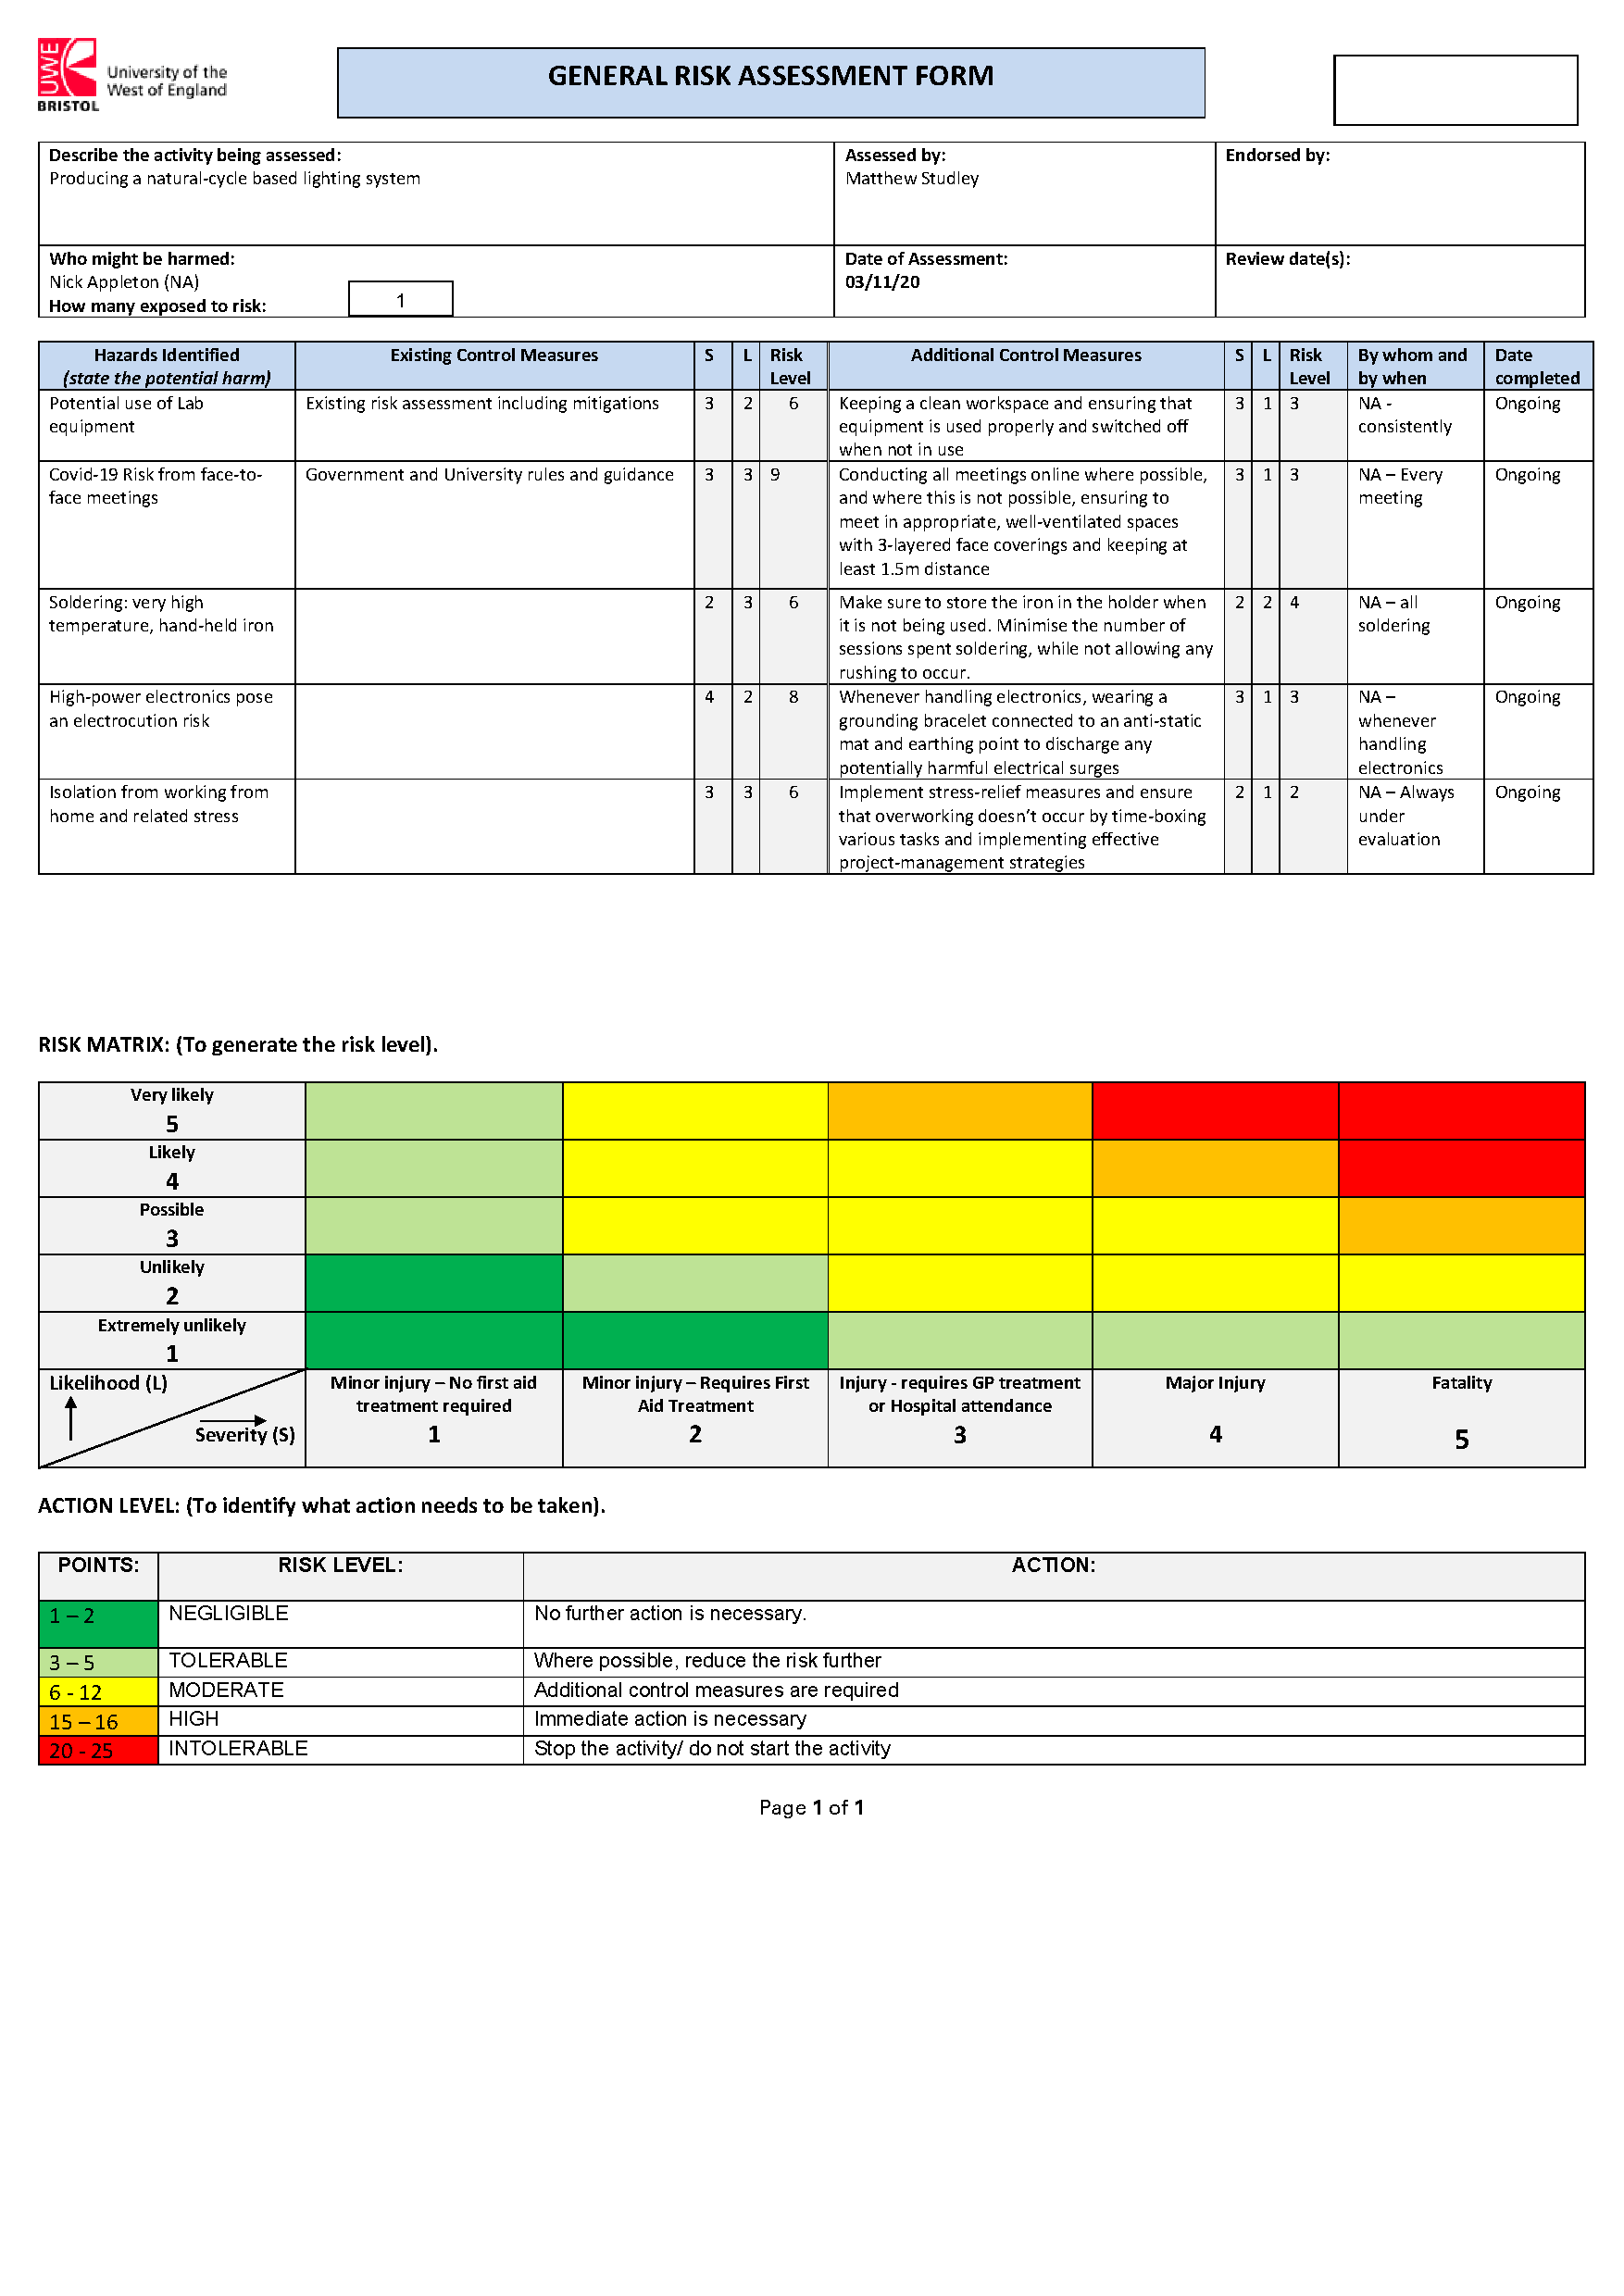
\includepdf[ offset=0 -120]{RiskAssessment.pdf}


\section{Security Form}
\label{appendix:security}
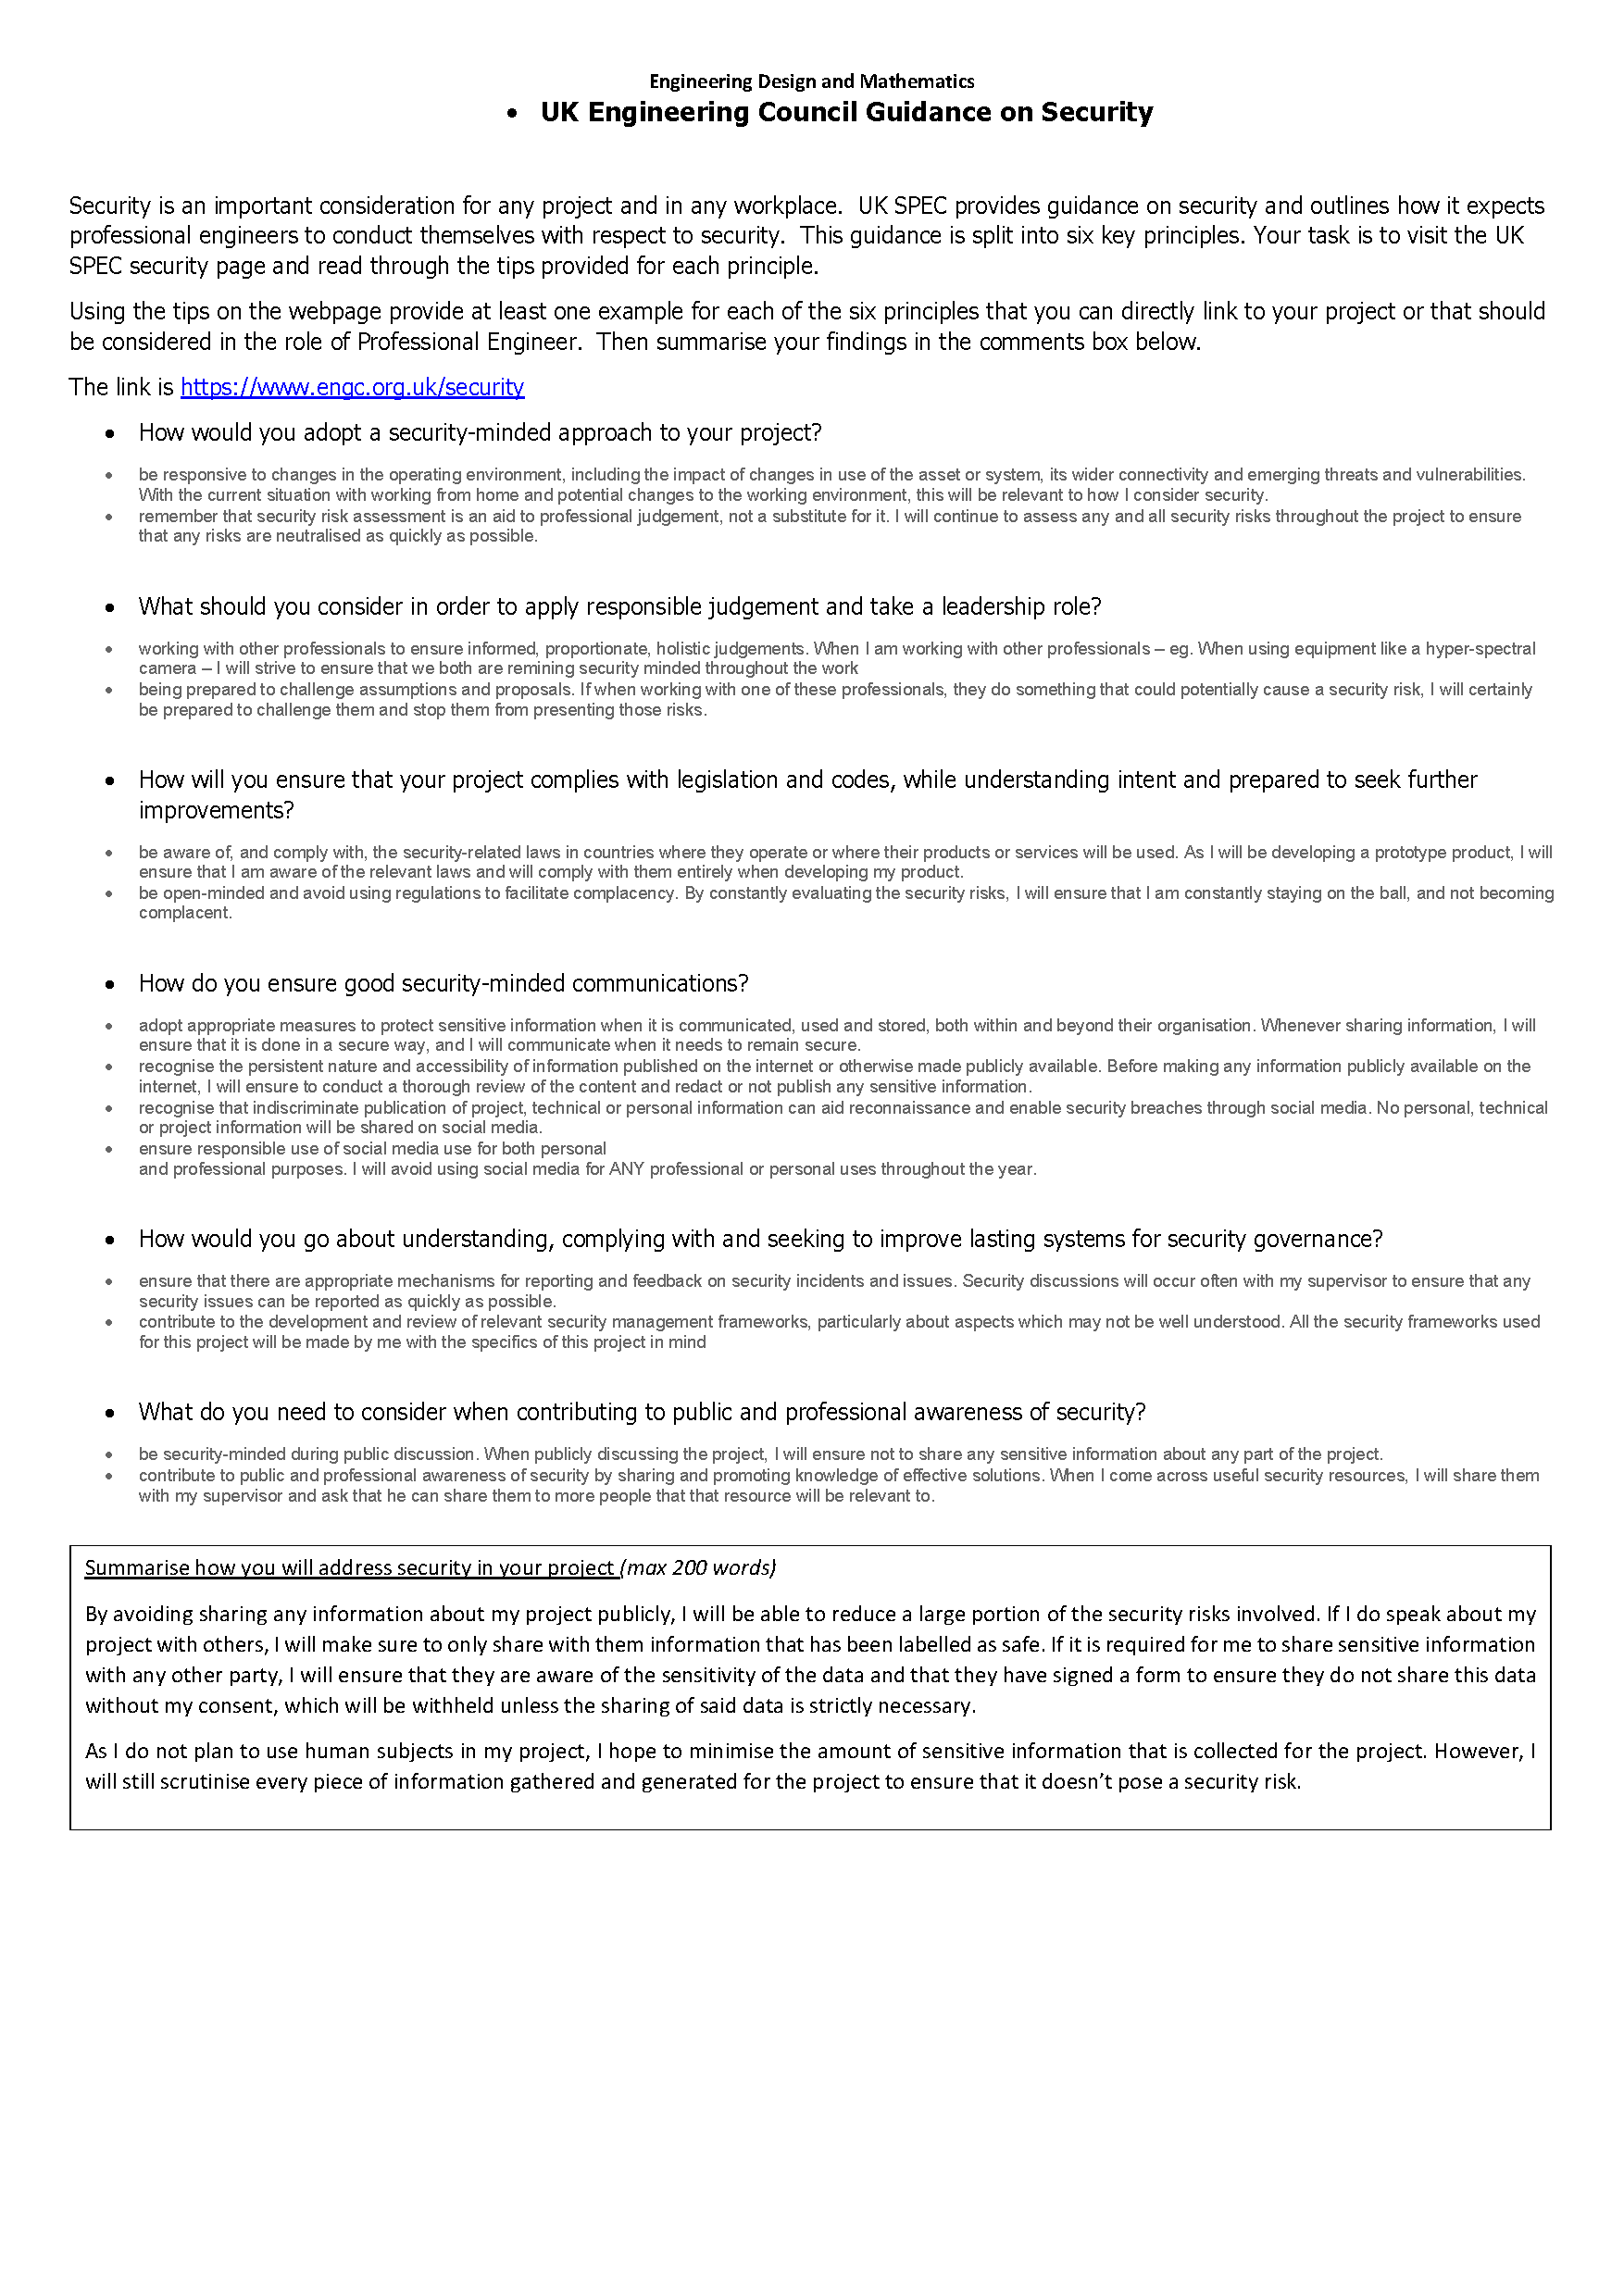
\includepdf[ offset=0 -100]{Security.pdf}


\section{Resources Form}
\label{appendix:resources}
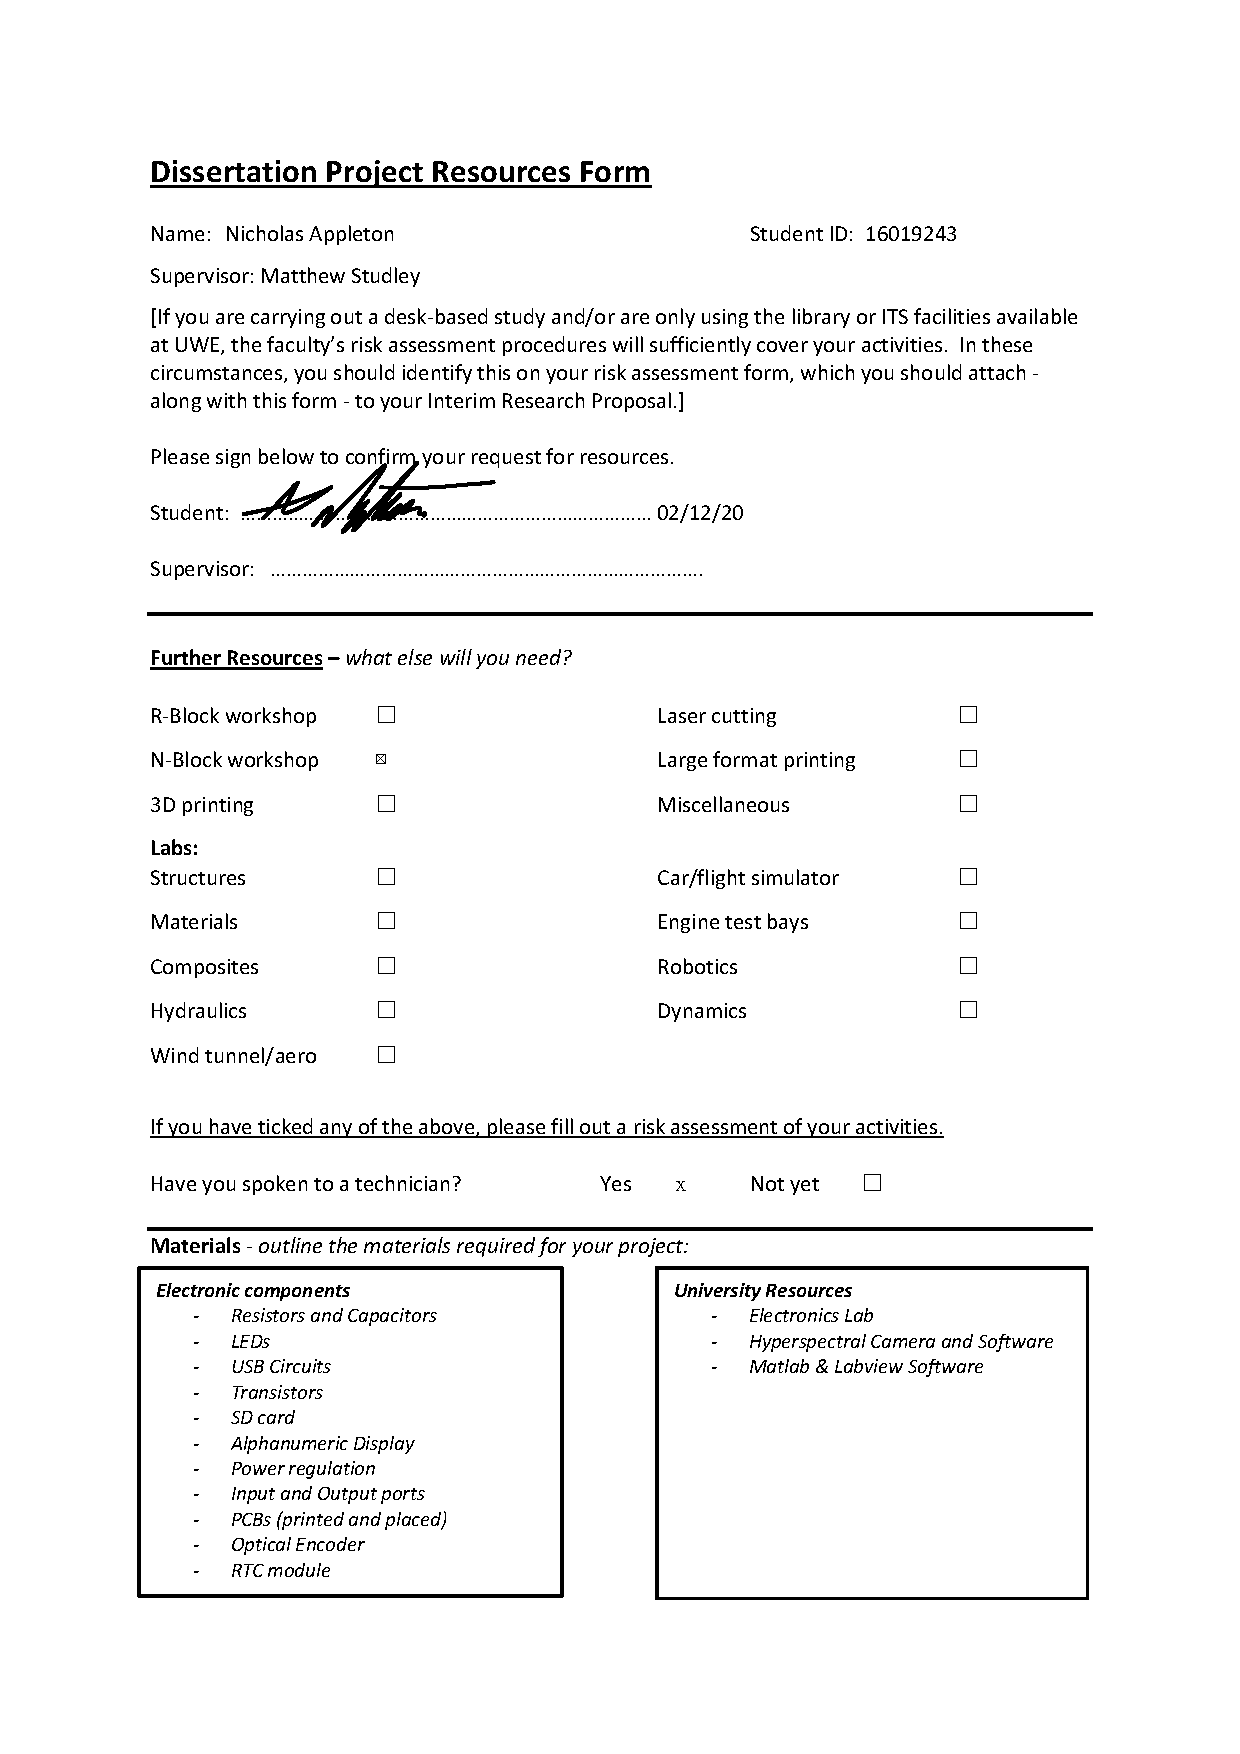
\includepdf[ offset=0 -40]{resources.pdf}

\section{Requirements Documentation}
\label{appendix:requirements}
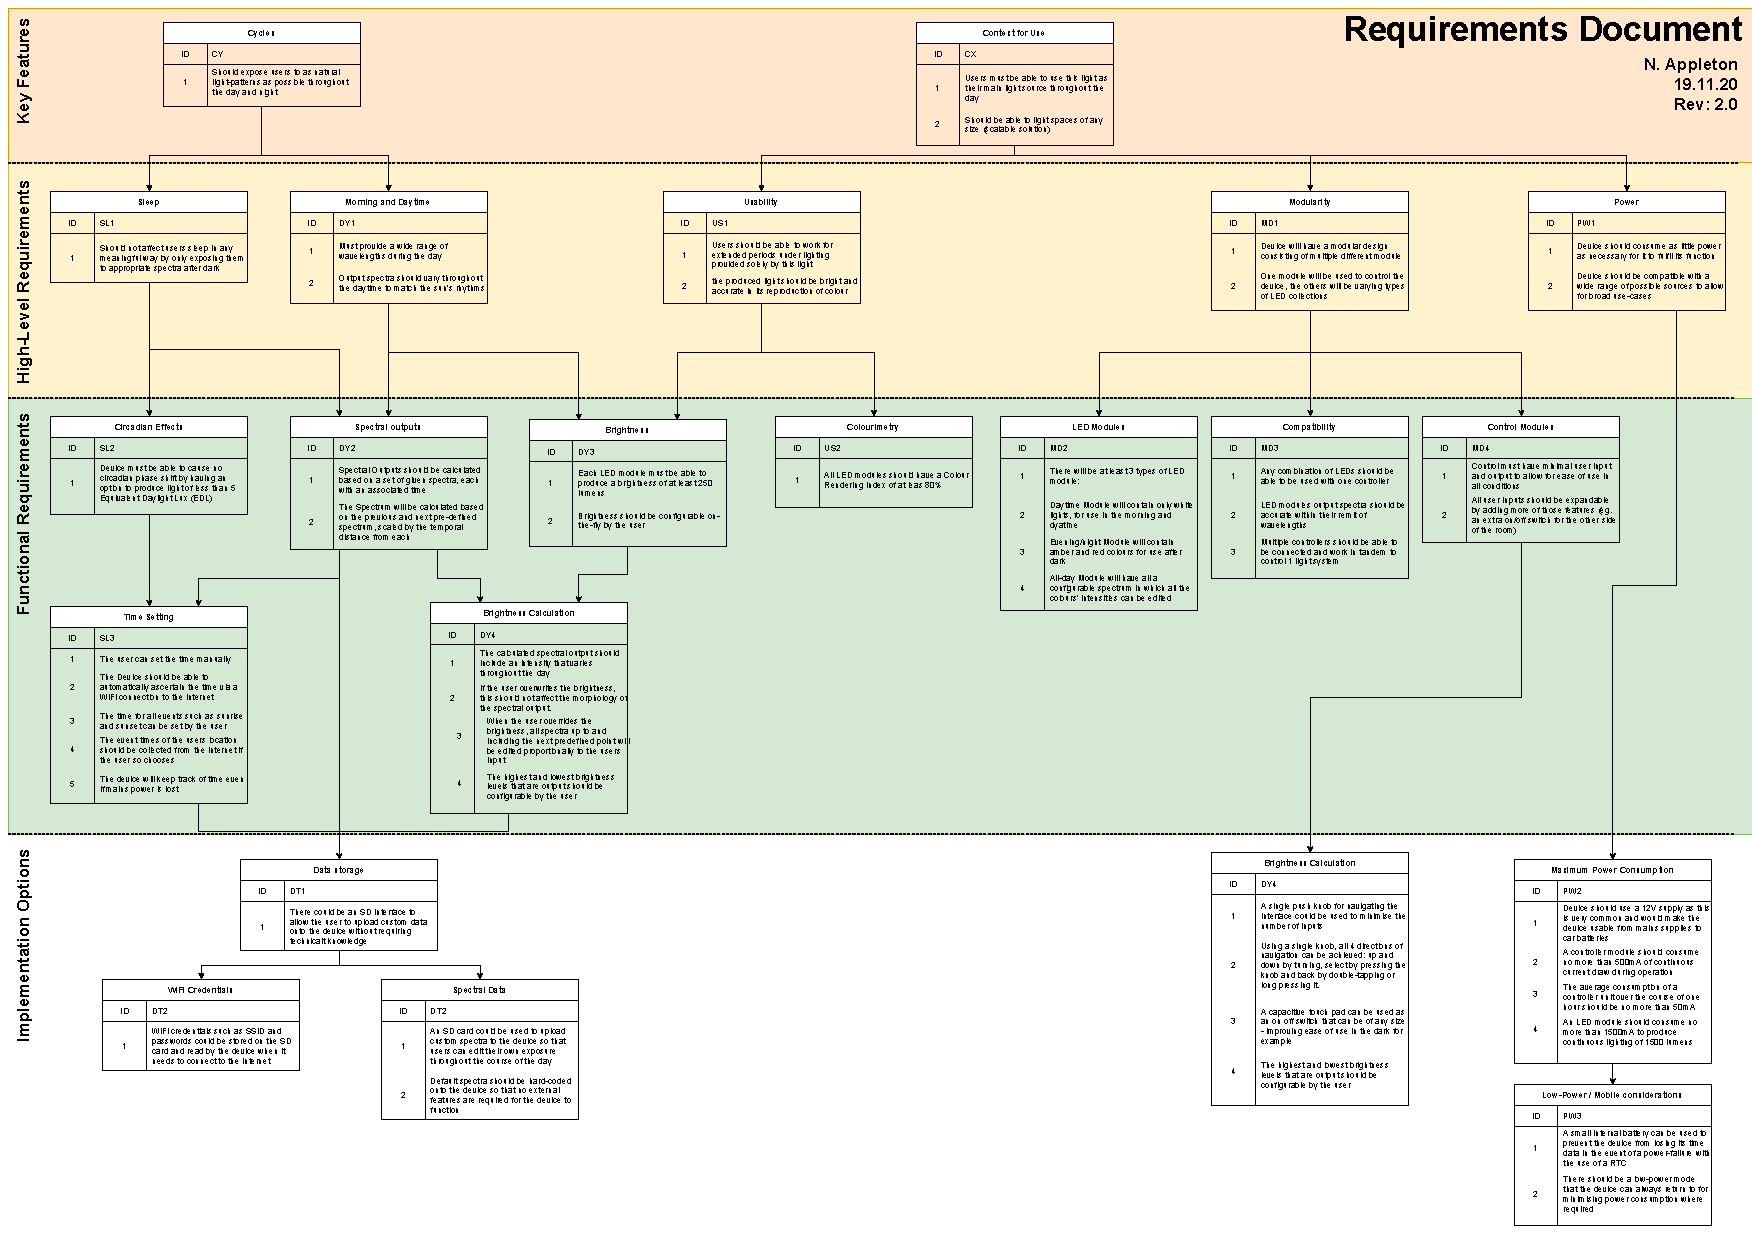
\includepdf[]{requirements.pdf}

\section{Gantt Charts}
\label{appendix:charts}
All Gantts as of 07-12-20
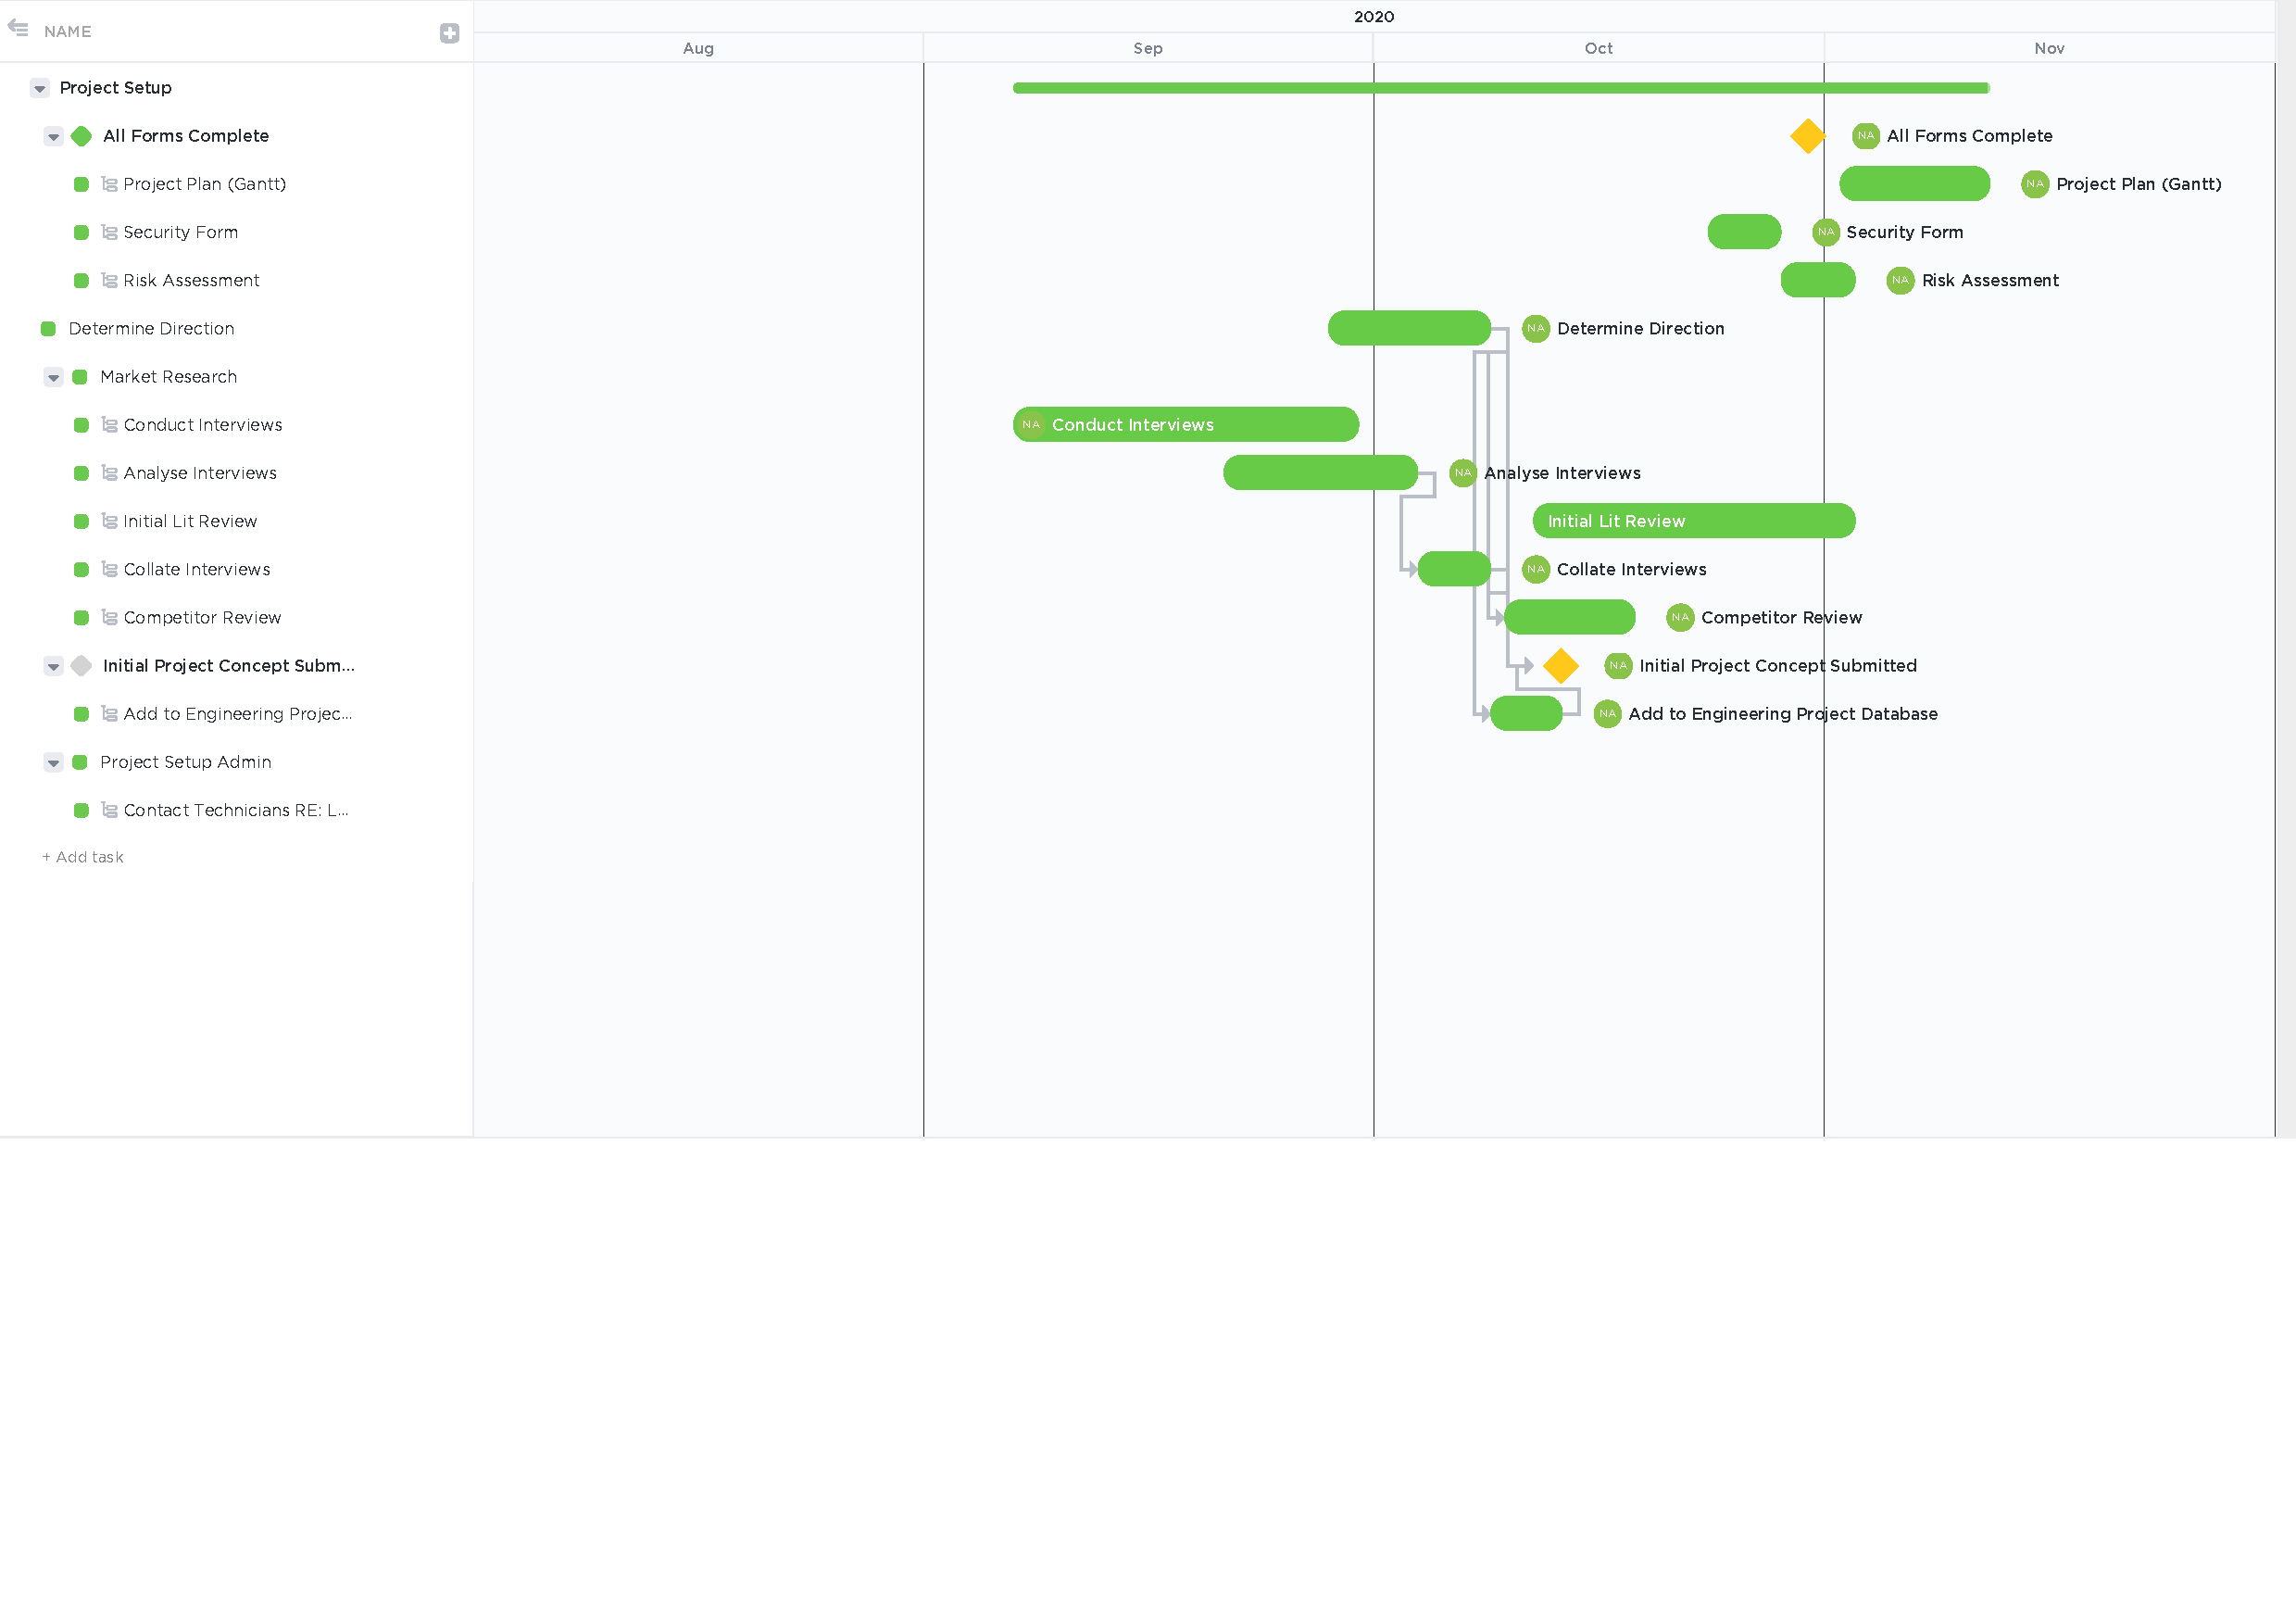
\includepdf{Gantts/Setup.pdf}
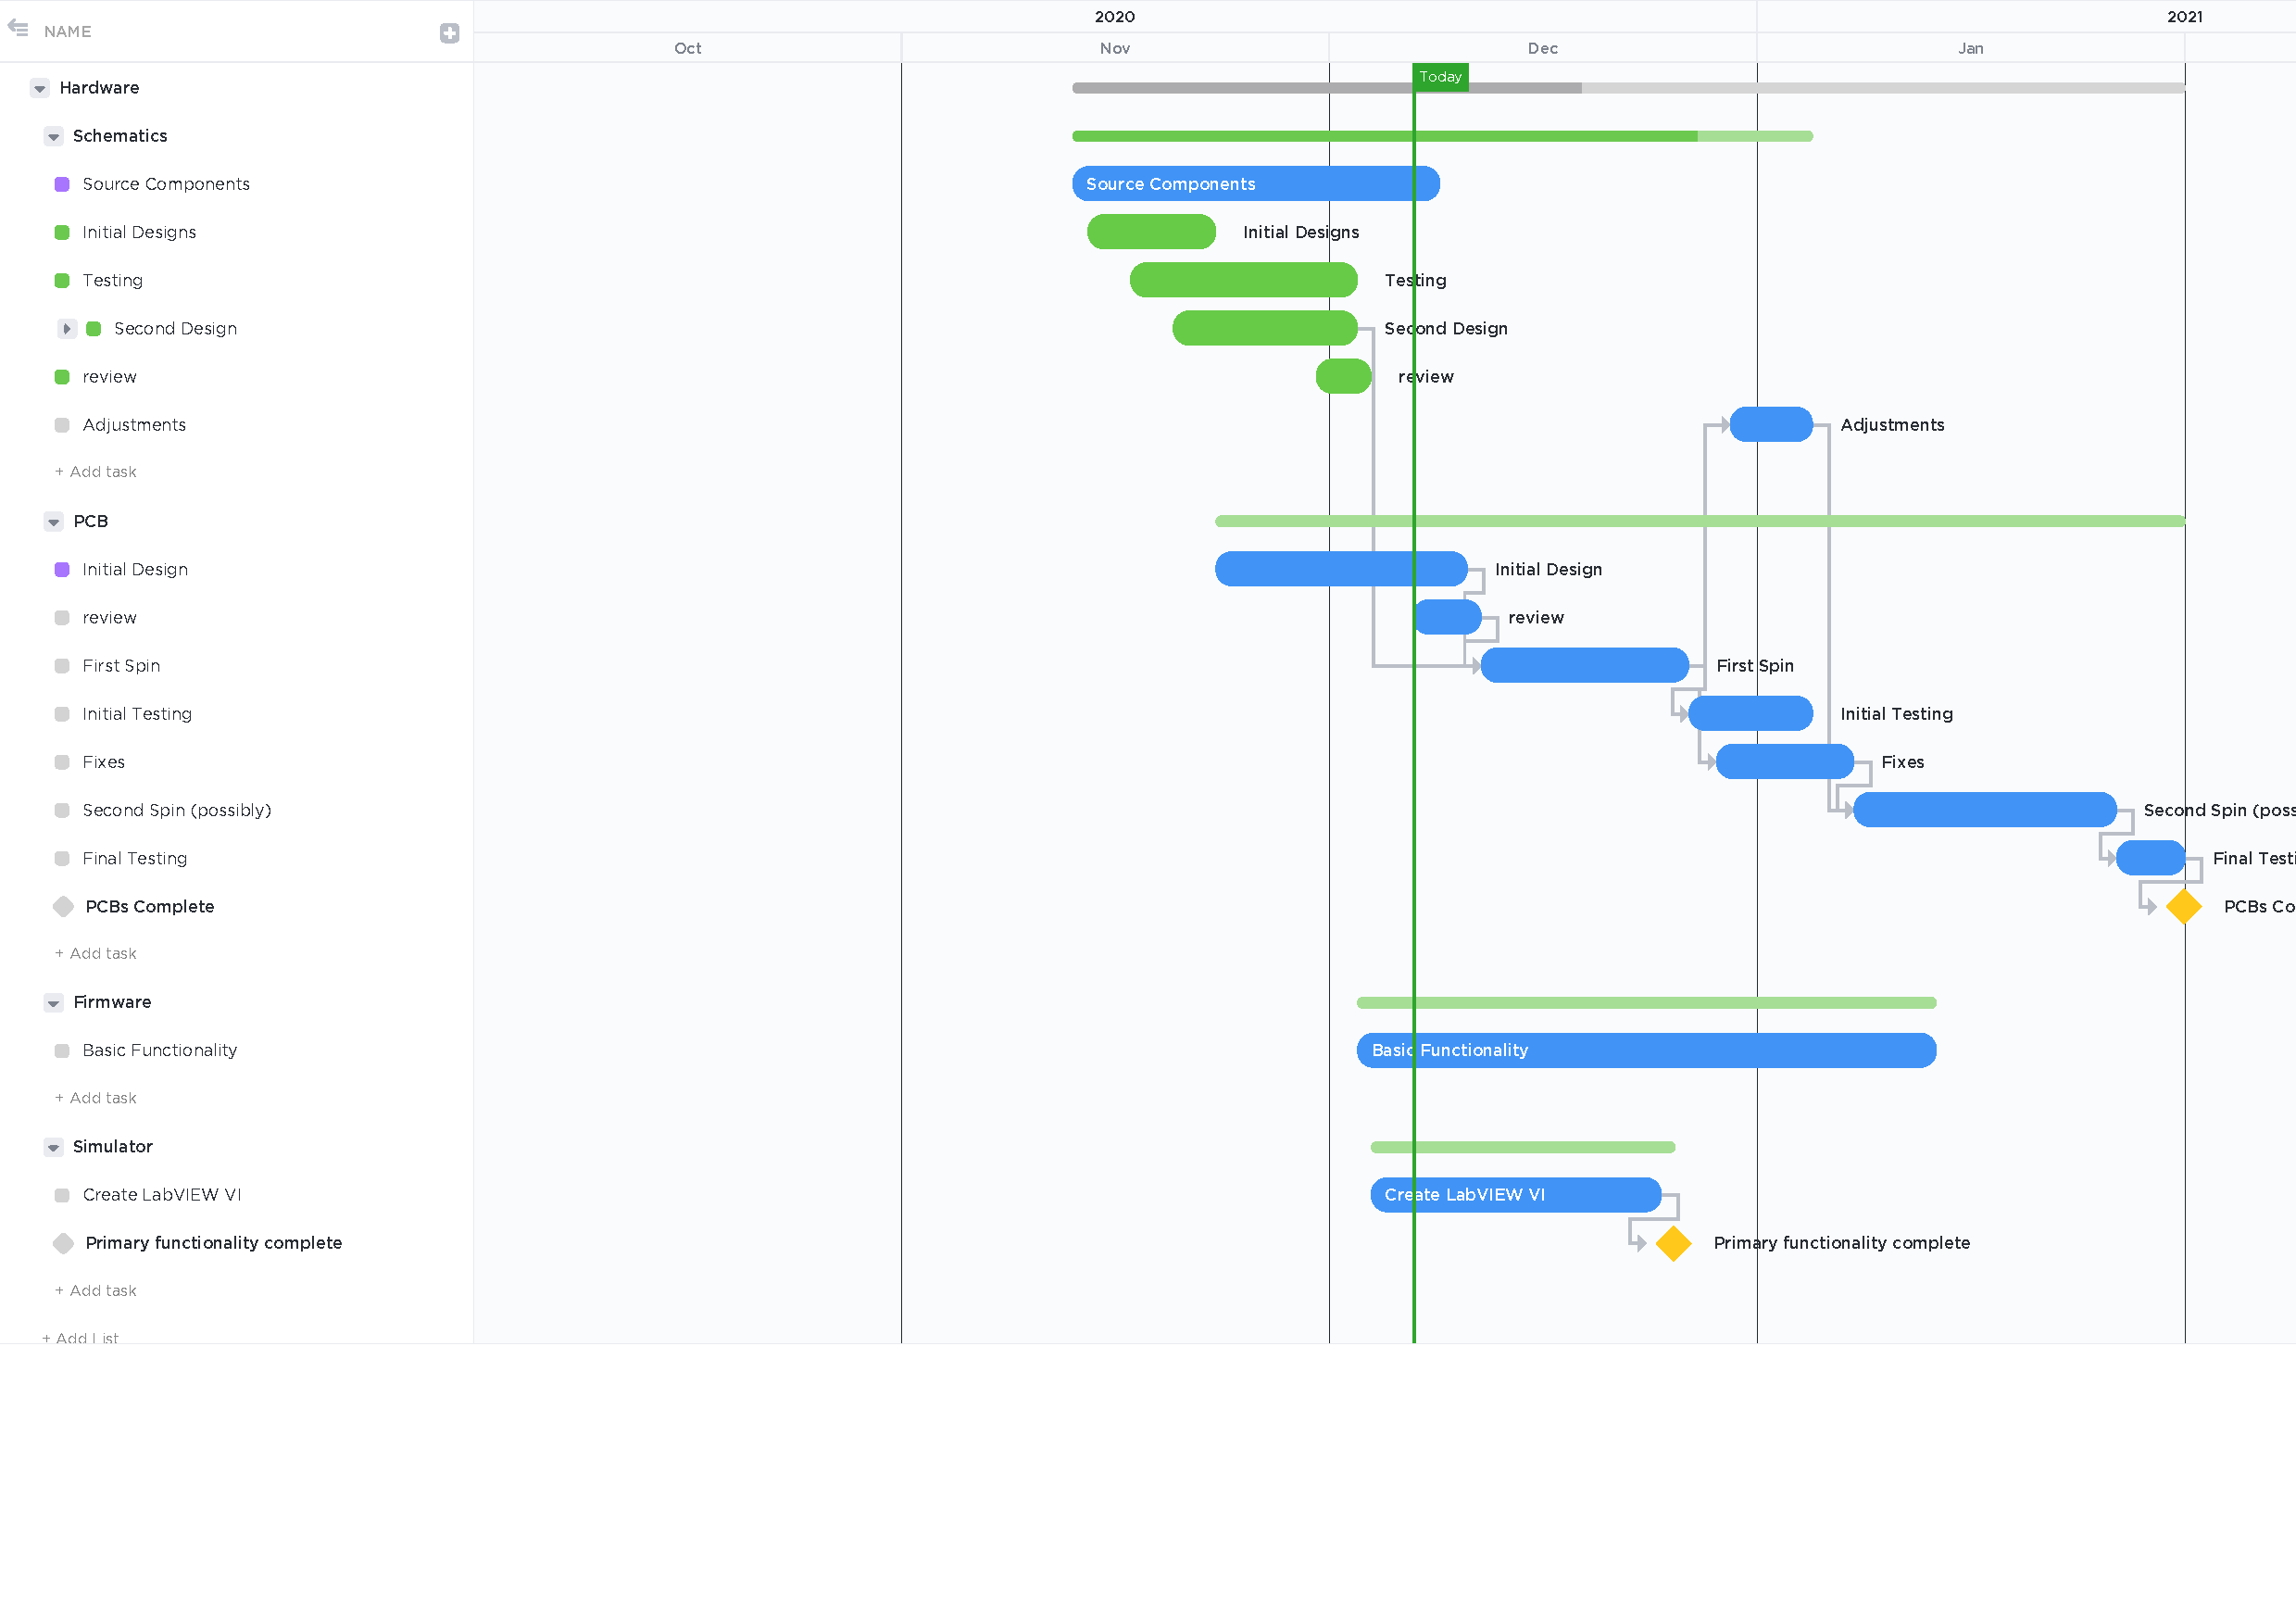
\includepdf{Gantts/Hardware.pdf}
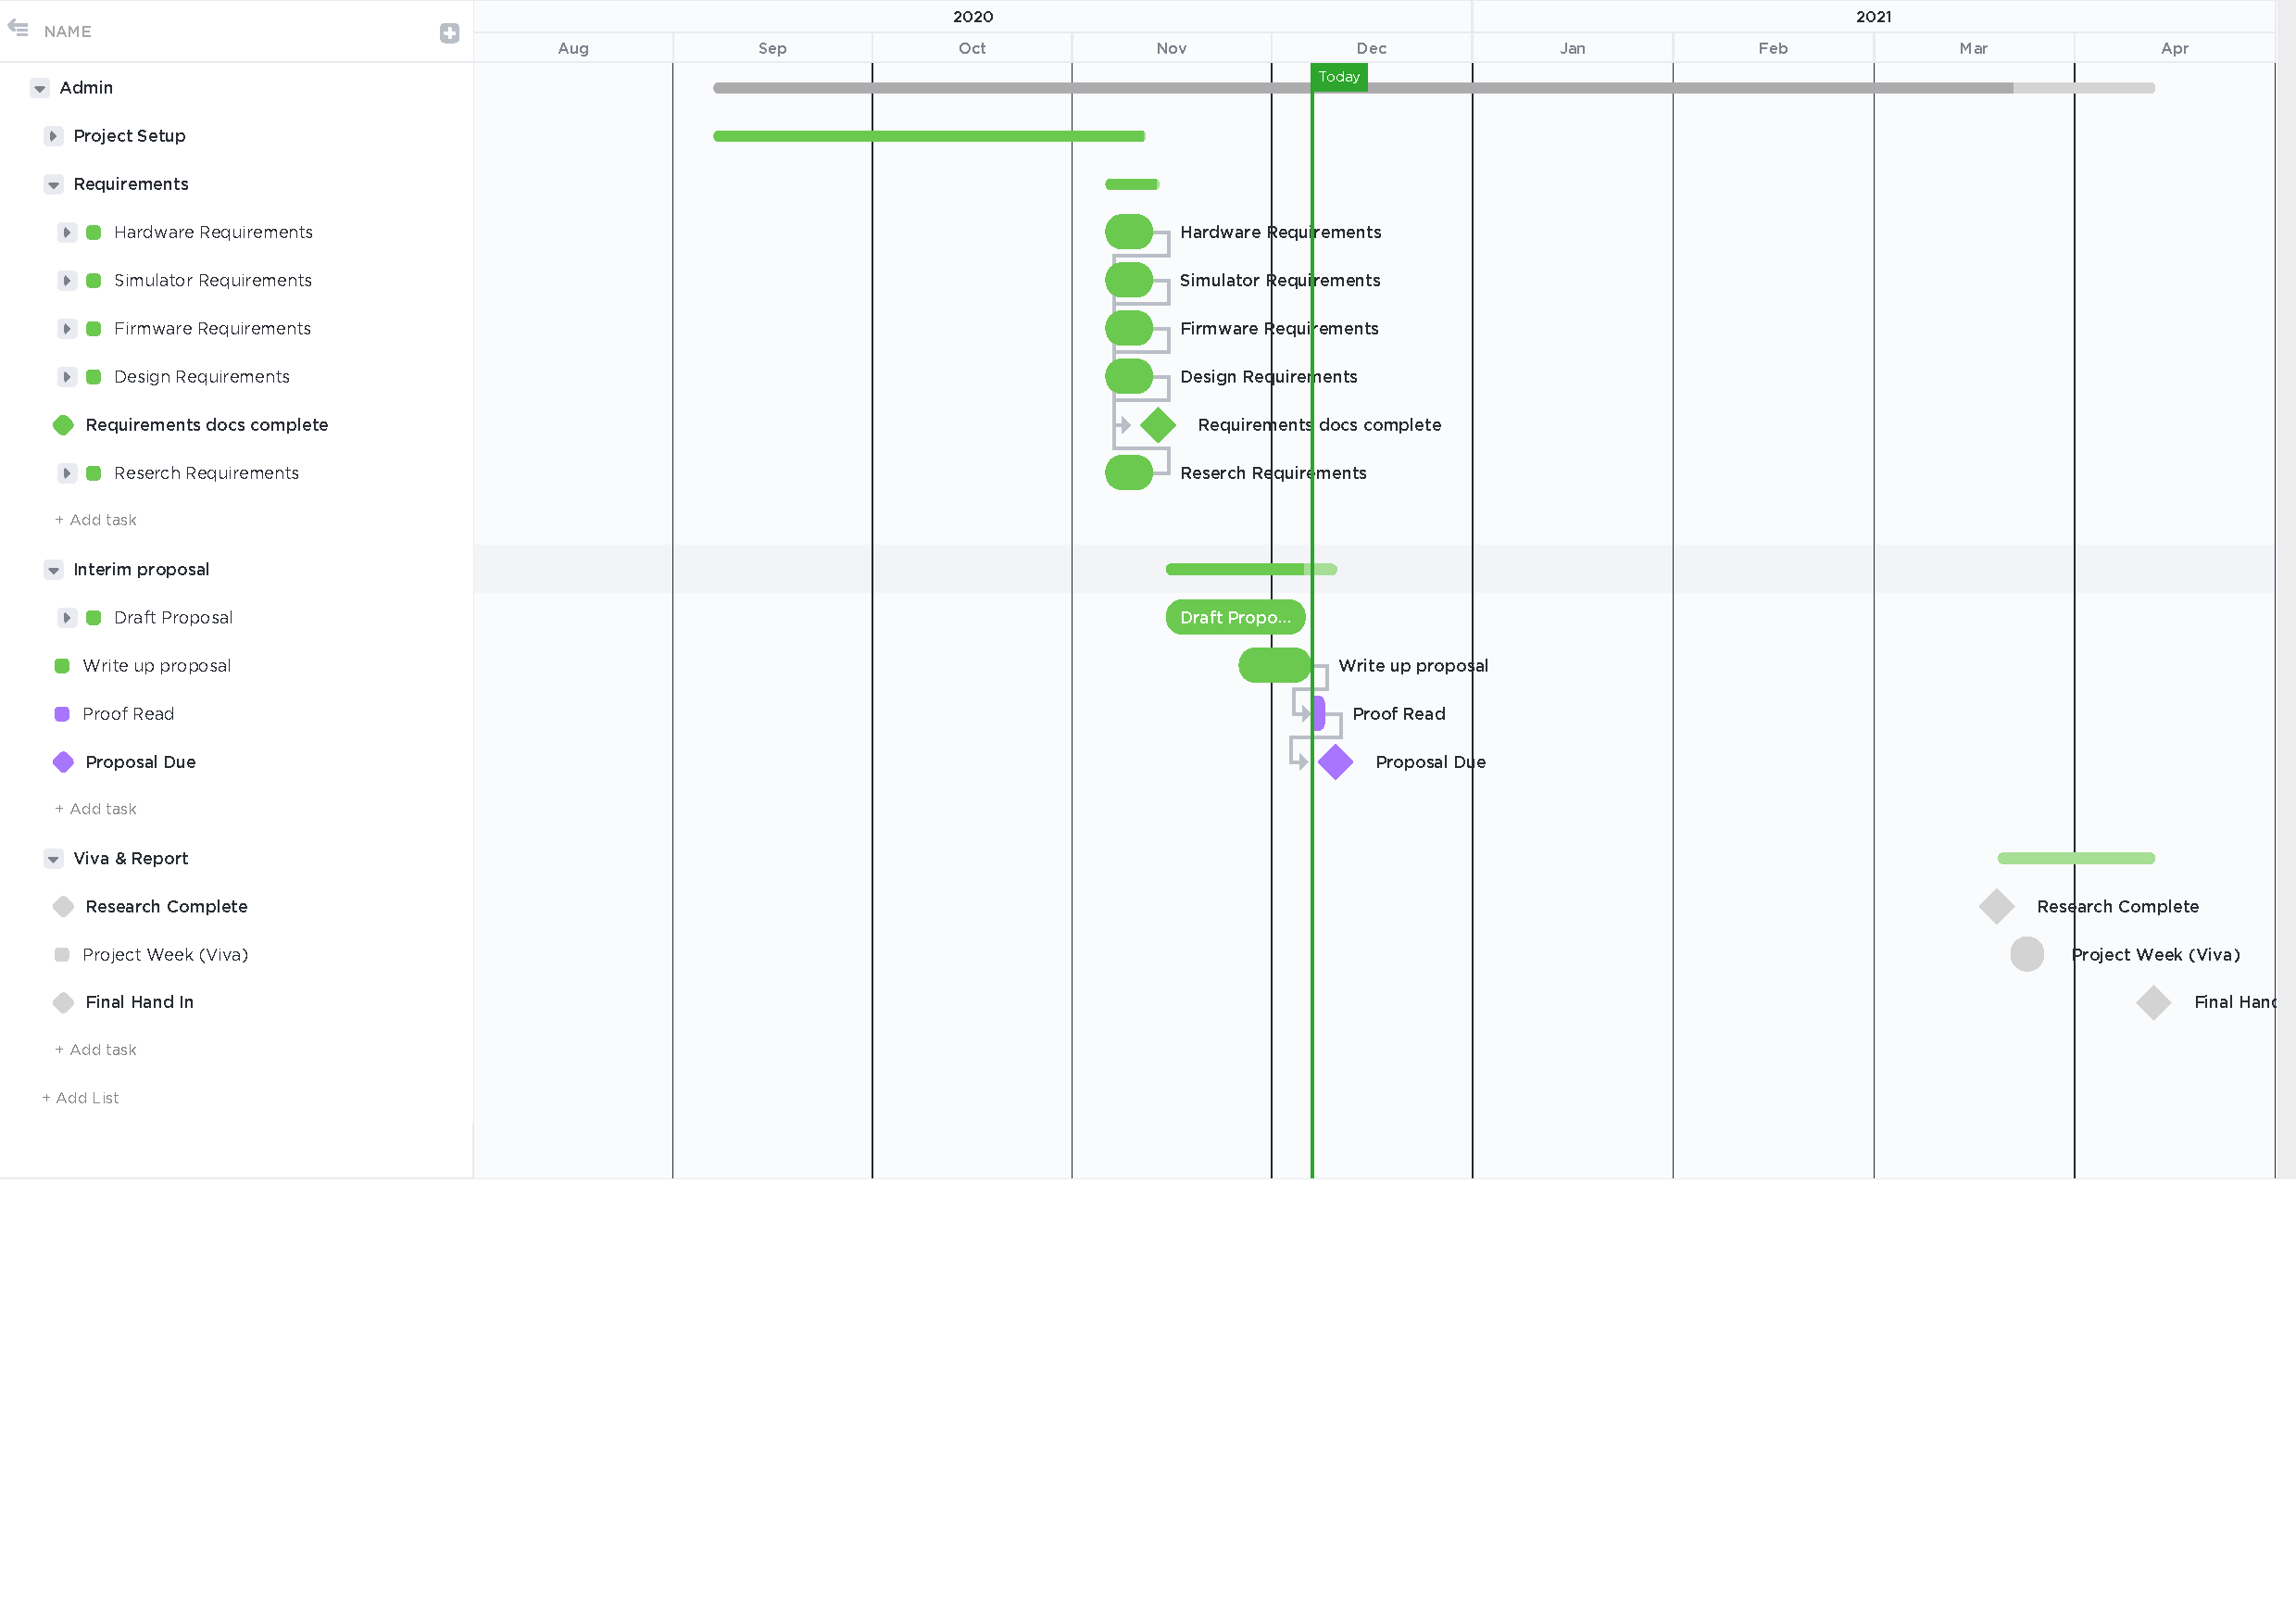
\includepdf{Gantts/Docs.pdf}
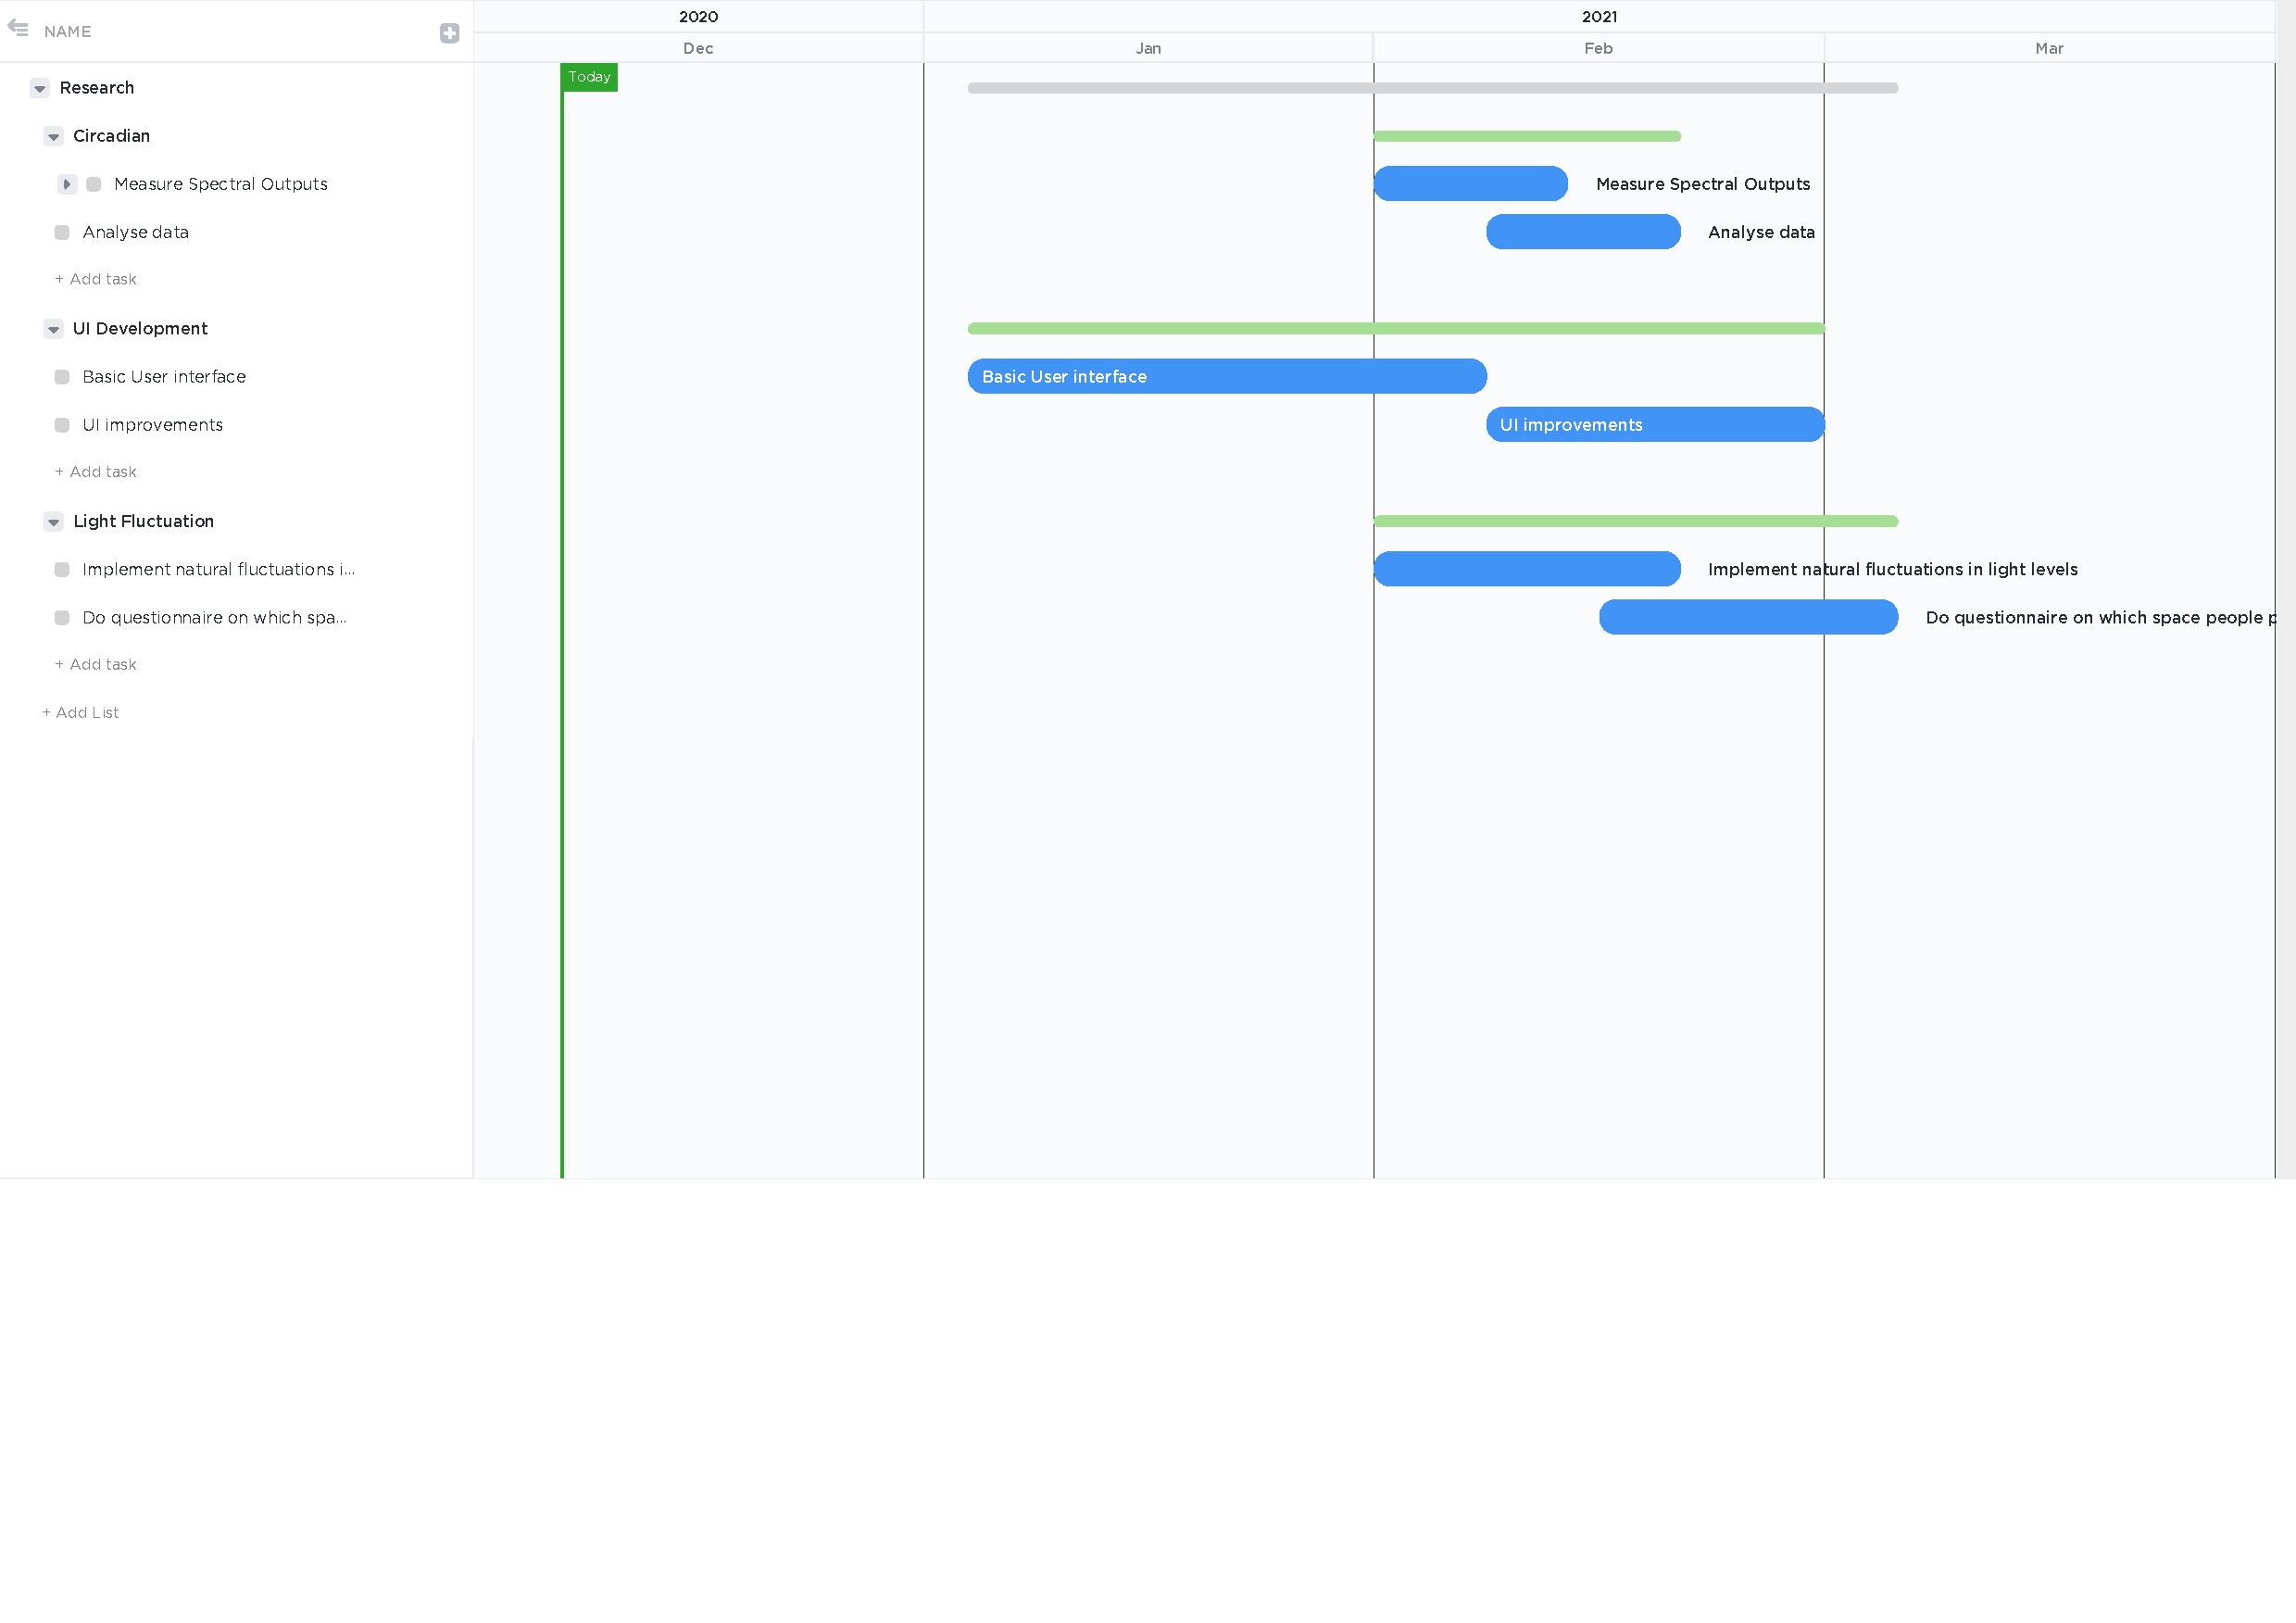
\includepdf{Gantts/Research.pdf}

%----------------------------------------------------------------------------------------

\end{document}
